\documentclass[conference]{IEEEtran}
\IEEEoverridecommandlockouts
% The preceding line is only needed to identify funding in the first footnote. If that is unneeded, please comment it out.
\usepackage{cite}
\usepackage[ngerman]{babel}
\usepackage[utf8]{inputenc}
\usepackage{amsmath,amssymb,amsfonts}
\usepackage{algorithmic}
\usepackage{graphicx}
\usepackage{textcomp}
\usepackage{xcolor}
\usepackage{listings}
\usepackage{bbold}


\definecolor{pblue}{rgb}{0.13,0.13,1}
\definecolor{pgreen}{rgb}{0,0.5,0}
\definecolor{pred}{rgb}{0.9,0,0}
\definecolor{pgrey}{rgb}{0.46,0.45,0.48}
\lstset{language=Python,
	showspaces=false,
	showtabs=false,
	breaklines=true,
	tabsize=2,
	showstringspaces=false,
	breakatwhitespace=true,
	commentstyle=\color{pgreen},
	keywordstyle=\color{pblue},
	stringstyle=\color{pred},
	basicstyle=\ttfamily
}


\usepackage{url}
\def\BibTeX{{\rm B\kern-.05em{\sc i\kern-.025em b}\kern-.08em
		T\kern-.1667em\lower.7ex\hbox{E}\kern-.125emX}}
\begin{document}
	
	\title{Videoanalyse und Objekttracking}
	
	\author{\IEEEauthorblockN{1\textsuperscript{st} Bartolovic Eduard}
		\IEEEauthorblockA{\textit{Hochschule München} \\
			München, Deutschland \\
			eduard.bartolovic0@hm.edu}
		\and
		\IEEEauthorblockN{2\textsuperscript{nd} Thomas Willeit}
		\IEEEauthorblockA{\textit{Hochschule München} \\
			München, Deutschland \\
			XXXXX@hm.edu}
		\and
		\IEEEauthorblockN{3\textsuperscript{rd} Schäfer Julia}
		\IEEEauthorblockA{\textit{Hochschule München} \\
			München, Deutschland \\
			j.schaefer0@hm.edu}
	}
	
	
	\maketitle
	
	\begin{abstract}
		
	\end{abstract}
	
	
	\section{Videomaterial}
	Für dieses Projekt wurden mehrere Aufnahmen aufgenommen. Ziel war es keine zu chaotischen aber auch nicht zu einfache Aufnahmen zu erstellen. Auch sollten verschiedene Szenarien abgebildet werden.\\
	\textbf{Verkehrsaufnahmen am Brudermühltunnel am Mittleren Ring:}\\
	Dieser Teil des Mittleren Rings ist sehr verkehrsreich und Autobahnähnlich ausgebaut. Es gibt mehrere Fahrspuren. Alle Fahrzeuge fahren im Sichtfeld in eine Richtung. Es sind ein paar Laternen und Bäume in der Aufnahme die die Sicht etwas beeinträchtigen. Es sind nur Pkwim Datensatz enthalten. Teilweise missachten Fahrzeuge den Sicherheitsabstand und fahren sehr nah aufeinander auf. Das Video hat 60 Bilder pro Sekunde und hat eine Bildauflösung $3840$ × $2160$. Es wurde kein Stativ verwendet sondern nur die interne Stabilisierung des Smartphones genutzt.
	\begin{figure}[!h]
		\begin{center}
			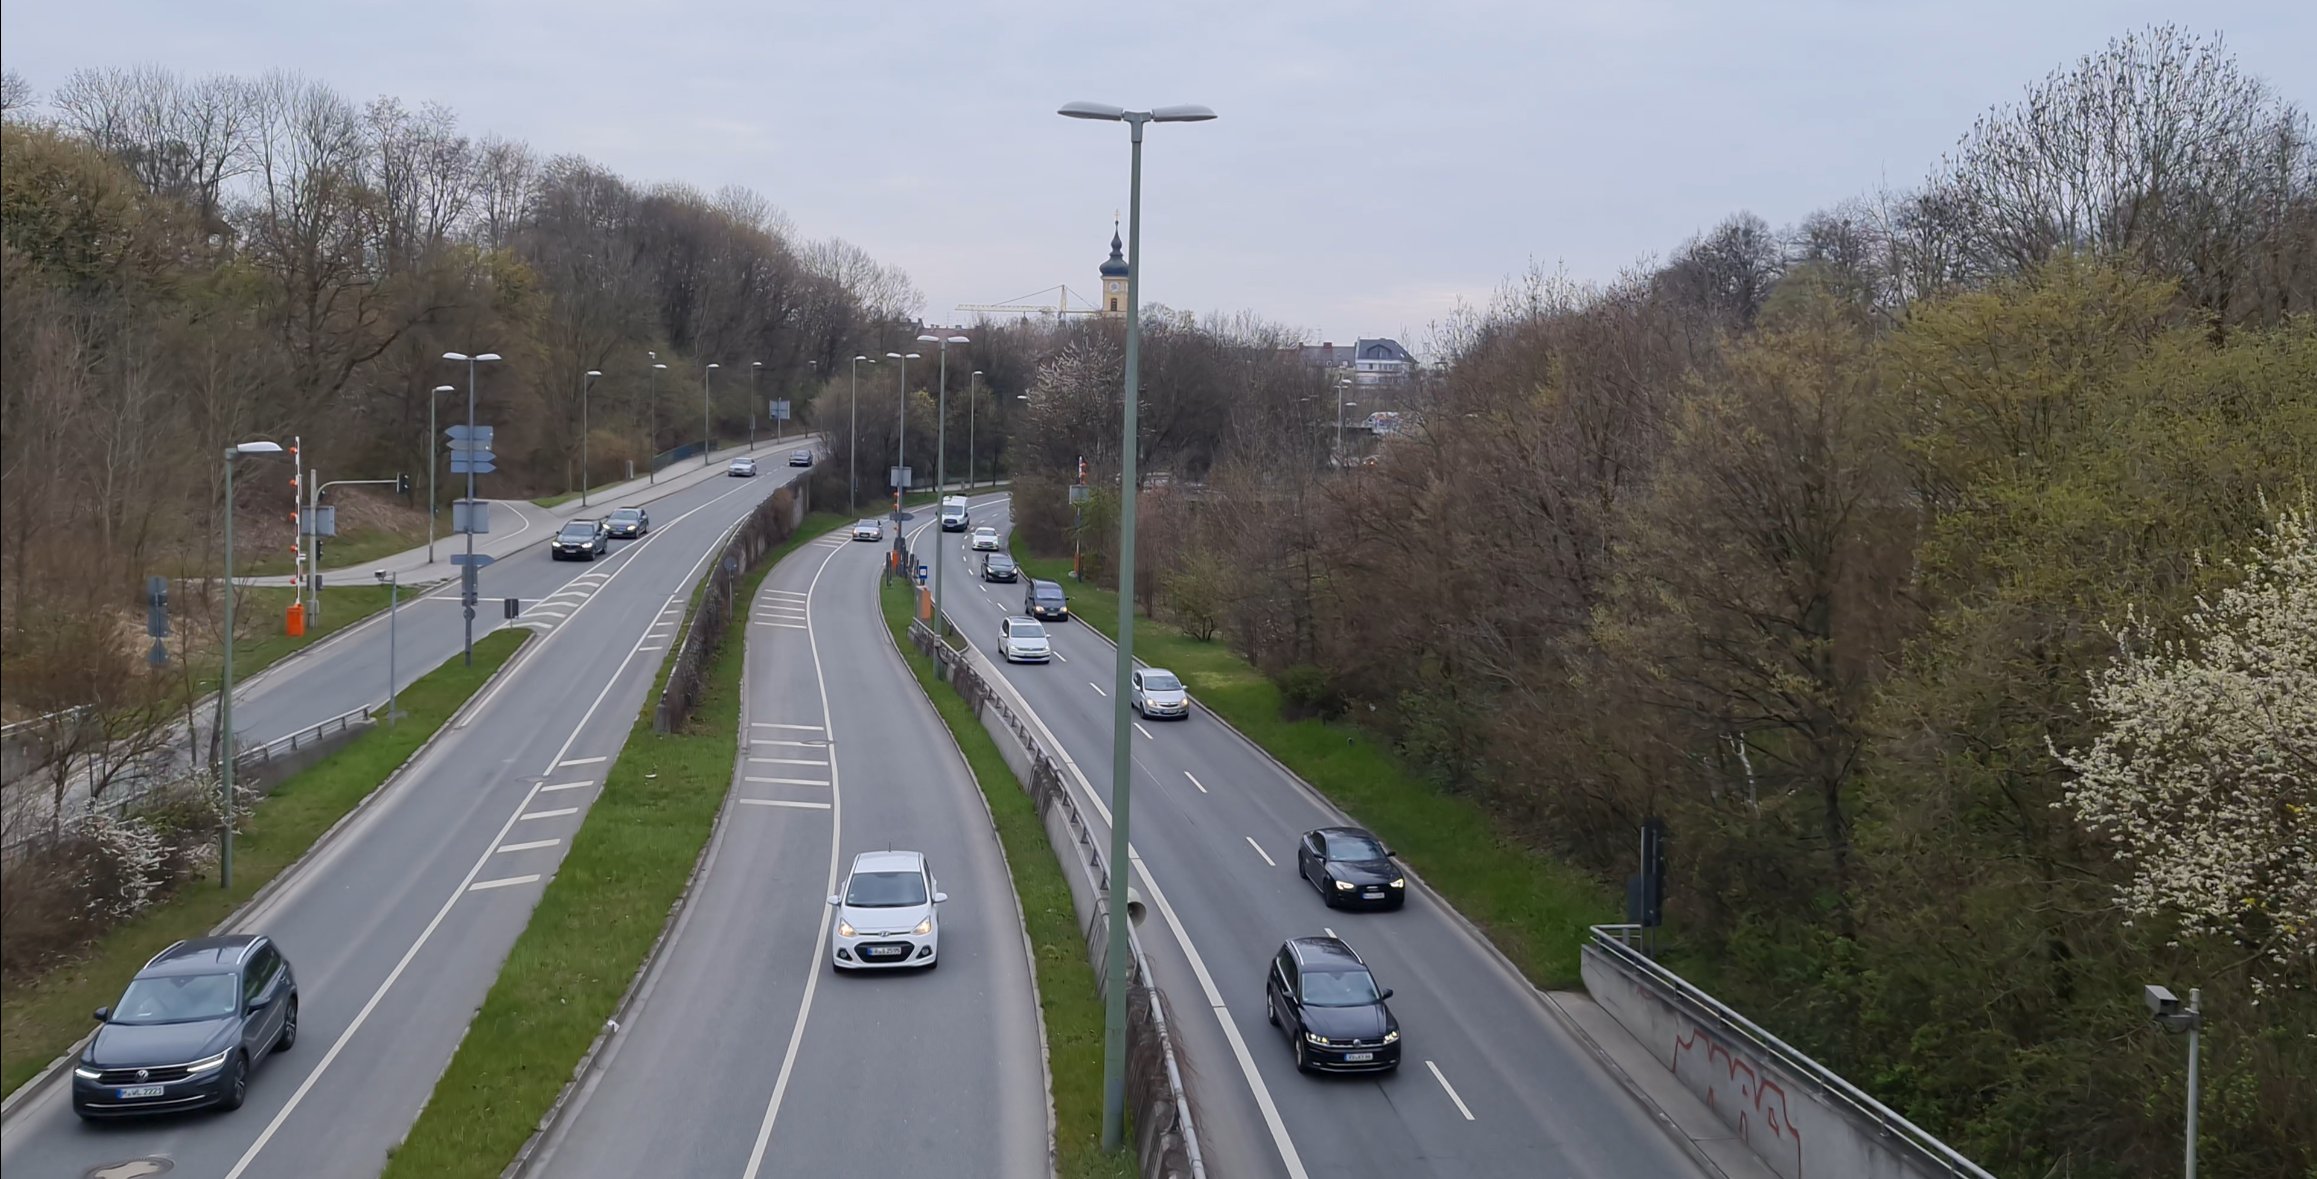
\includegraphics[width=7cm]{Media/BrudermuhlRaw.png}
			\caption{Verkehrsaufnahmen am Brudermühltunnel}
			\label{BrudermuhlRaw}
		\end{center}
	\end{figure}\\
	\textbf{Verkehrsaufnahmen am Candidtunnel:}\\
	Eine stark befahrene Straße mit einer viel zahl von Verkehrsteilnehmern. Es herrscht zwei Richtungsverkehr mit insgesamt sechs Fahrspuren. In eine Richtung stehen die Fahrzeuge in einem Stau. Durch Regen spiegeln viele Oberflächen. Die Bäume bewegen sich aufgrund von stärkeren Wind und verdecken einen Teil der Fahrbahn. Diese Aufnahme ist die Anspruchsvollste. In diesem Video sind neben Pkw auch Busse enthalten. Das Video hat 60 Bilder pro Sekunde und hat eine Bildauflösung $3840$ × $2160$. Es wurde kein Stativ verwendet sondern nur die interne Stabilisierung des Smartphones genutzt.
	\begin{figure}[!h]
		\begin{center}
			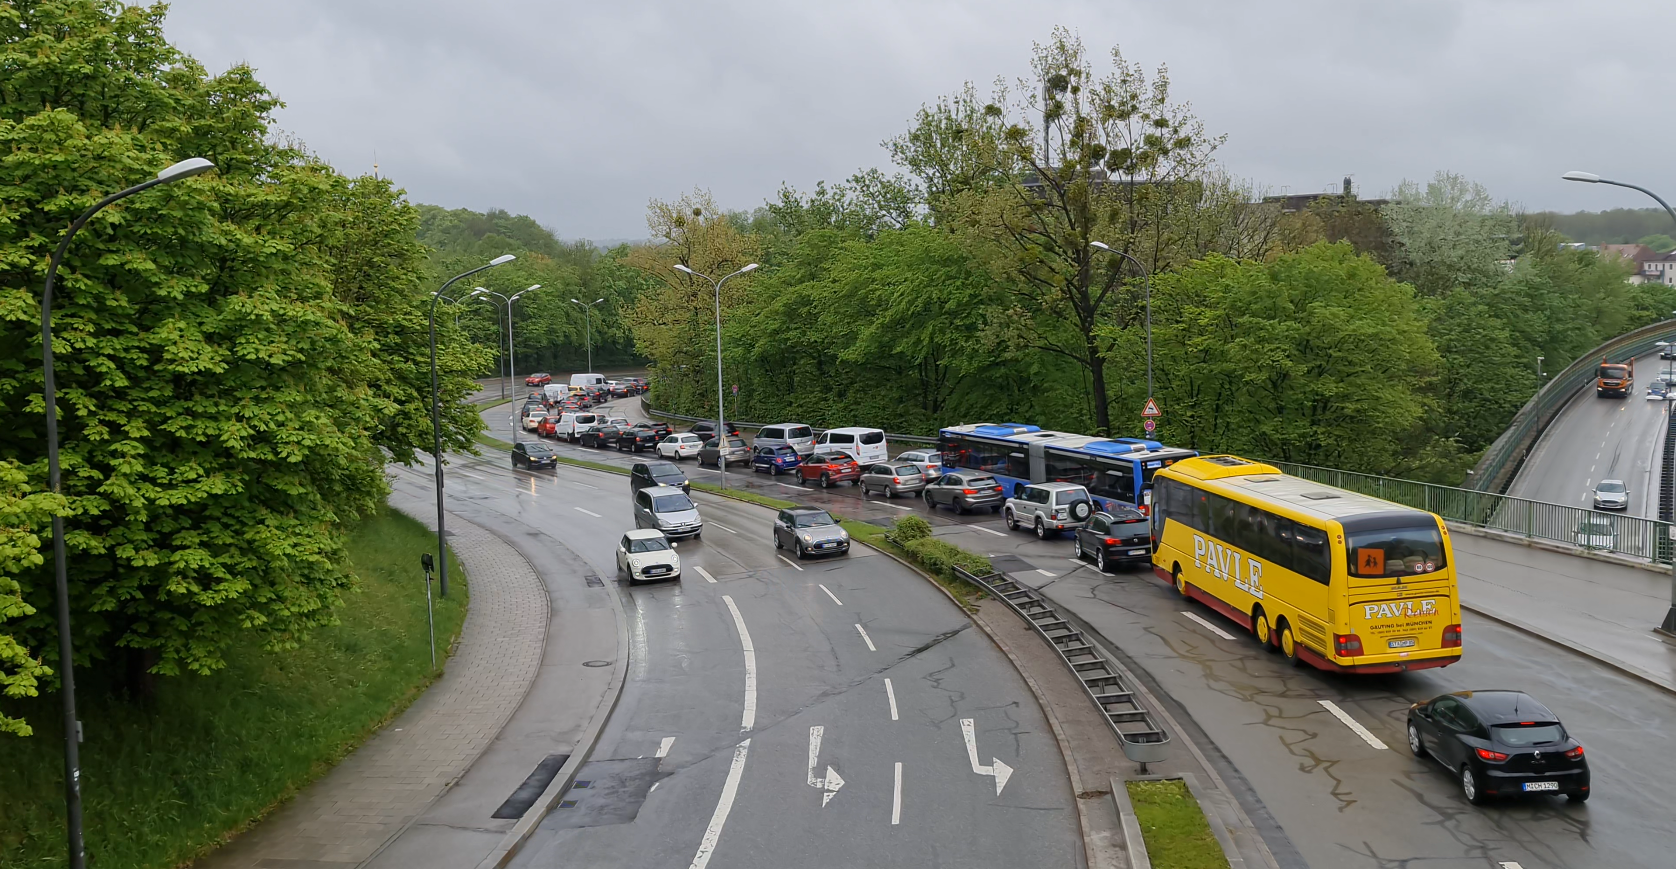
\includegraphics[width=7cm]{Media/CandidRaw.png}
			\caption{Verkehrsaufnahmen am Candidtunnel.}
			\label{BrudermuhlRaw}
		\end{center}
	\end{figure}\\
	\textbf{Zugaufnahmen an der Donnersbergerbrücke:}\\
	Eine Aufnahme der einer der am stärksten befahren Bahnstrecken Europas \cite{z1}. Hier existiert viel Zugverkehr auf mehreren Gleisen mit unterschiedlichen Zugtypen. Beobachtet werden die vier Gleise der zwei Bahnsteige der S-Bahnhalts Donnersbergerbrücke. Ein Hindernis sind die Masten, Signale und das Bahnsteigdach welche einen guten Blick auf die Züge erschweren. In dieser Aufnahme sind Züge und Fußgänger enthalten. Der Fokus liegt aber bei den Zügen. Das Video hat 30 Bilder pro Sekunde und hat eine Bildauflösung $1920$ × $1080$. Es wurde ein Stativ verwendet.
	\begin{figure}[!h]
		\begin{center}
			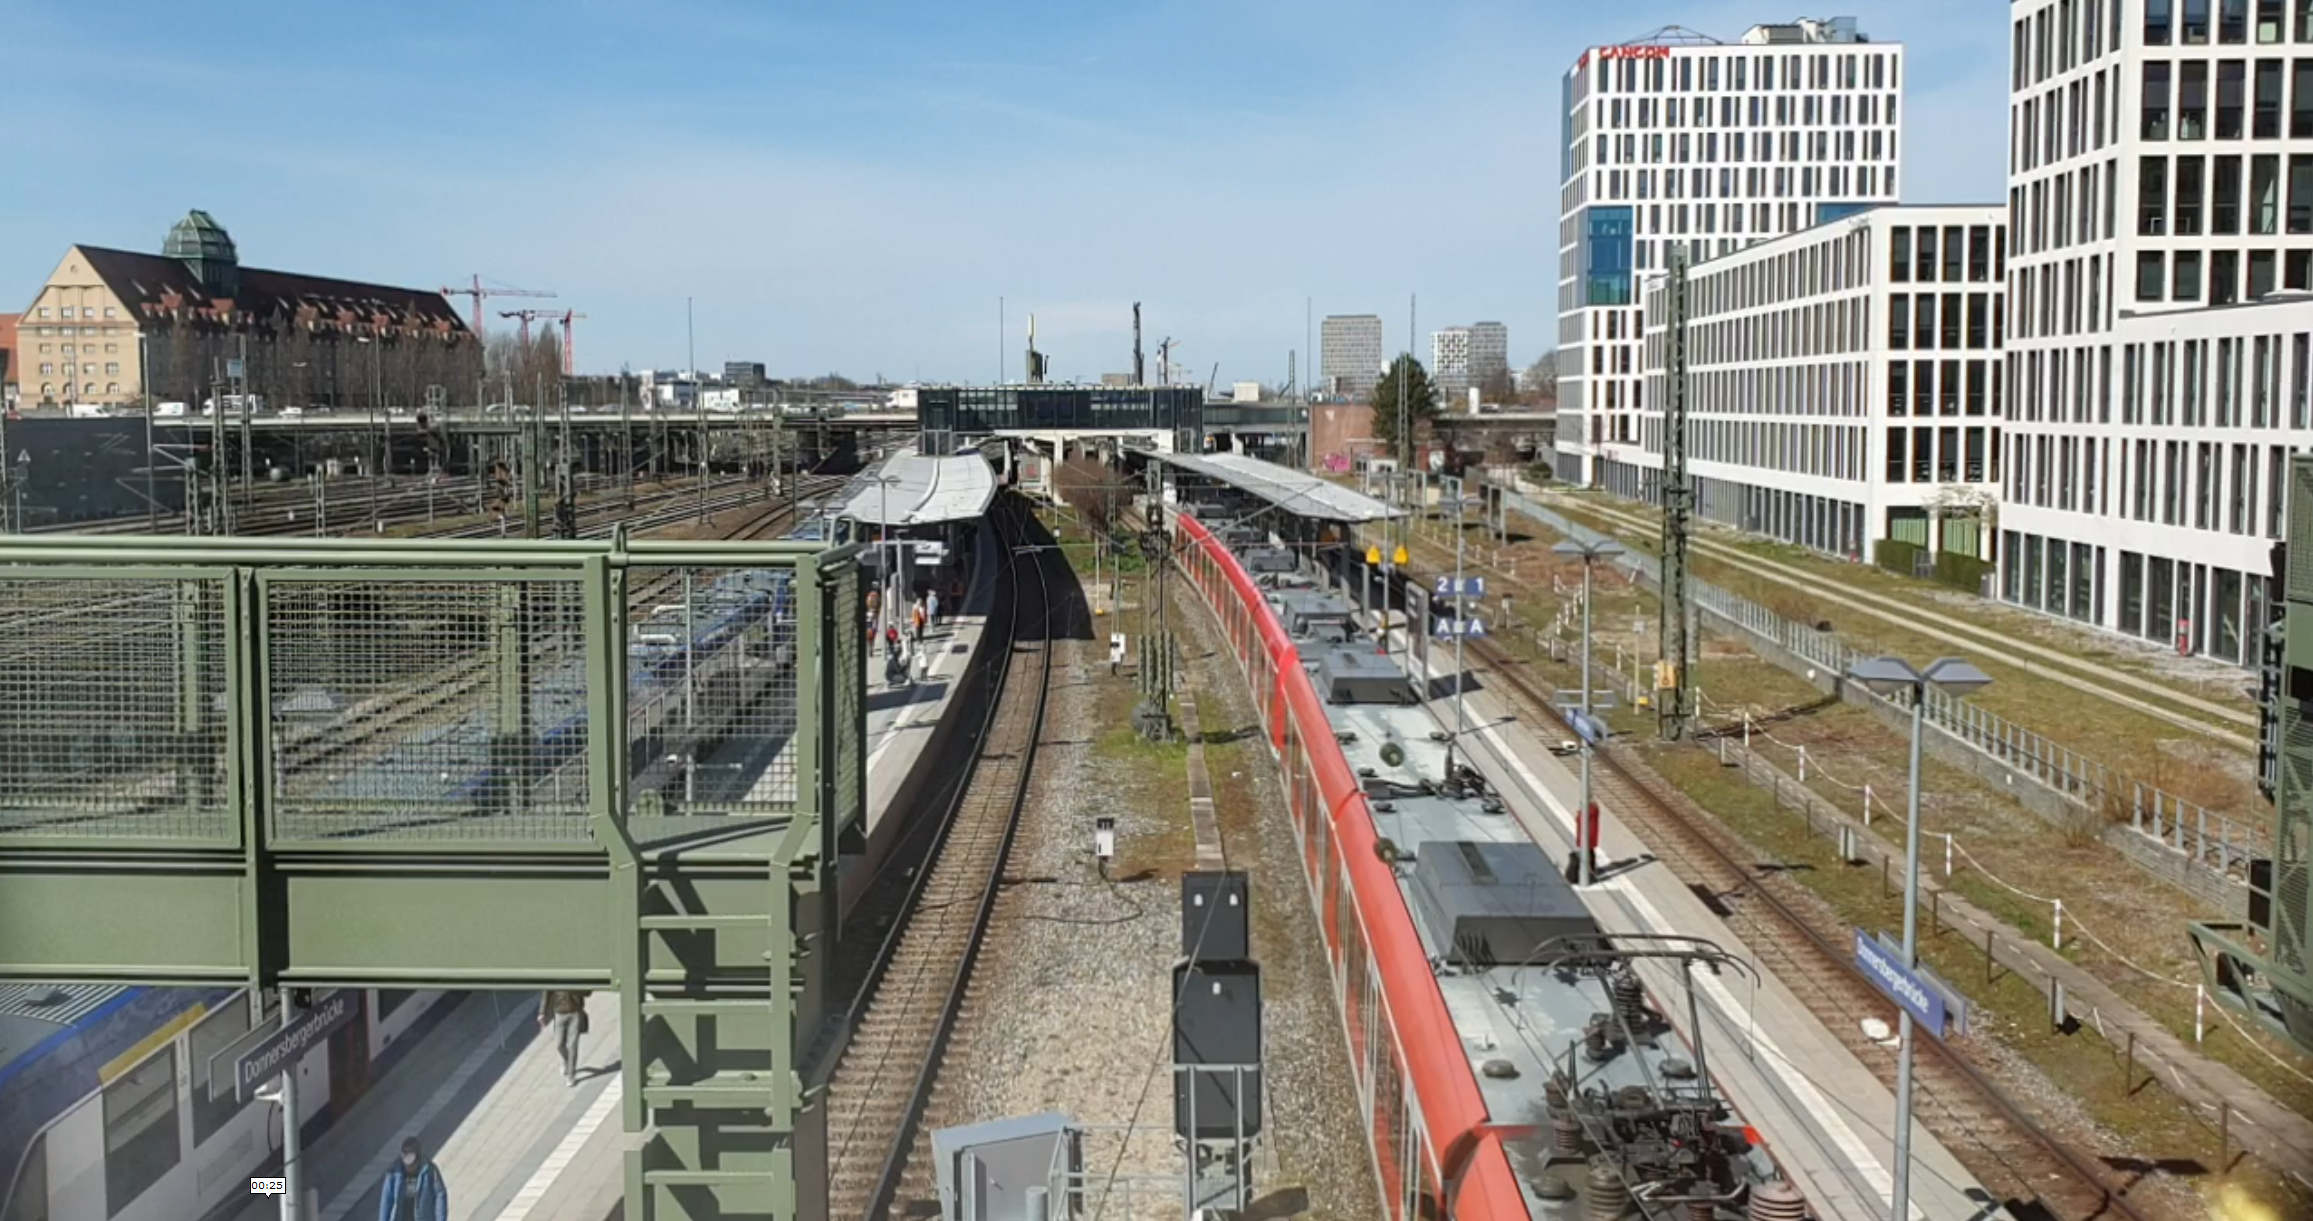
\includegraphics[width=7cm]{Media/DonnersbergerRaw.png}
			\caption{Zugaufnahmen an der Donnersbergerbrücke}
			\label{BrudermuhlRaw}
		\end{center}
	\end{figure}
	
	\section{Konzept}
	
	\begin{figure*}[!h]
		\begin{center}
			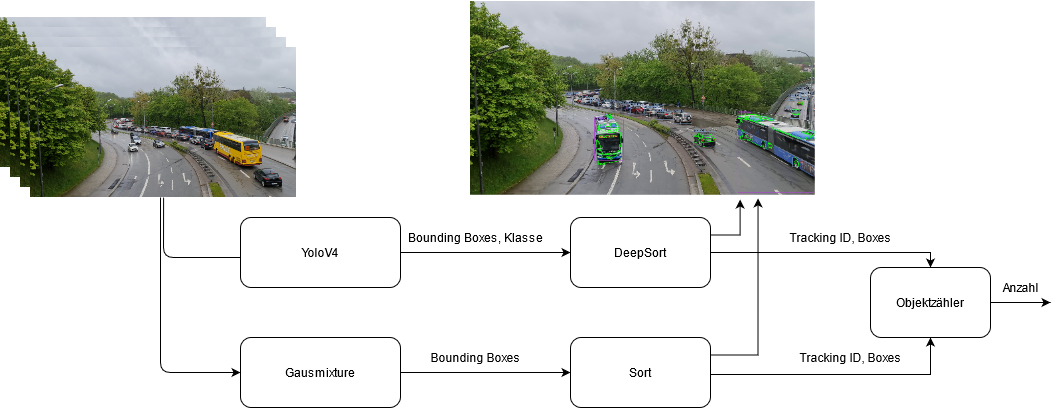
\includegraphics[width=16cm]{Media/KonzeptVAOT.png}
			\caption{Konzept für das Projekt}
			\label{Konzept}
		\end{center}
	\end{figure*}
	Ziel des Projektes ist es klassische Verfahren mit neueren DeepLearning Methoden zu vergleichen.
	Dafür ist für beide Arten eine Pipeline geschaffen worden.\\
	Für die Klassische Methoden wurde für die Objekterkennung das Gausmixture Verfahren verwendet und für das Tracking den SORT Algorithmus. Für die DeepLearning Verfahren wurde für die Objekterkennung ein Neuronales Netz  und für das Tracking wurde Deepsort verwendet.\\
	Mit einem Objektzähler können am Ende der beiden Pipelines die Objekte gezählt oder mit einer Zustandserkennung die Bewegungen und Stillstand erfasst werden. Die Abbildung \ref{Konzept} visualisiert das Konzept.\\
	\\
	Bilder werden mittels der OpenCV Bibliotheksmethoden Frame für Frame aus einem Video ausgelesen. Des weiteren ist es möglich Bilder vor der weiteren Verarbeitung noch beliebig zuzuschneiden um nur relevant Bereiche zu betrachten. Dies hat den Vorteil das die Performance steigt und auch die Genauigkeit mancher Algorithmen zunimmt. Diese Bilder werden dann in die Pipeline gelegt.\\
	Es muss die Objektzählerbox definiert werden.
	
	\section{Objekterkennung: Gauß Mixture}
	
	\subsection{Rauschminderung}
	
	\section{Objekterkennung: YoloV4}
	YOLO ist ein Neuronal Netz für die Echtzeit-Objekterkennung. In diesem Projekt verwendeten wir die 4te und damit aktuellste Version von Yolo\cite{b2}. So bietet jede Version inkrementelle Verbesserung zum jeweiligen Vorgänger. In dem folgenden Abschnitt werden die wichtigsten Punkte aller Versionen erläutert.\\
	YOLO ist die Abkürzung für 'You Only Look Once' was übersetzt 'Man sieht nur einmal hin' heißt. Die Aufgabe der Objekterkennung besteht darin, den Ort und die Größe der Bounding Box im Bild zu bestimmen, sowie die Objekte zu klassifizieren. Frühere Methoden, wie R-CNN und seine Variationen, verwendeten eine Pipeline, um diese Aufgabe in mehreren Schritten durchzuführen. Dies ist in der Ausführung langsam und aufwendiger zu trainieren, da jede einzelne Komponente separat trainiert werden muss. YOLO, erledigt beide Aufgaben mit einem einzigen Convolutional Neural Network. Es betrachtet dabei die Objekterkennung als ein Regressionsproblem auf räumlich getrennte Bounding Boxes und zugehörige Klassenwahrscheinlichkeiten.\\
	Die verwendete Loss-Funktion betrachtet drei Komponenten:
	\begin{enumerate}
		\item \textbf{Localization loss:} Differenz zwischen vorhergesagten Bounding-Box-Werten (x,y,w und h) und tatsächlichen Bounding-Box-Werten.
		\[ \lambda_{coord} \sum_{i=0}^{S^2}\sum_{j=0}^{B} \mathbb{1}_{i j}^{obj} [(x_i - \hat{x}_i )^2 + (y_i - \hat{y}_i )^2] \]
		\[ + \lambda_{coord} \sum_{i=0}^{S^2}\sum_{j=0}^{B} \mathbb{1}_{i j}^{obj} [(\sqrt{w_i} - \sqrt{\hat{w}_i} )^2 + (\sqrt{h_i} - \sqrt{\hat{h}_i} )^2] \]
		Wenn $\mathbb{1}_{i}^{obj} = 1$ dann ist die Boundingbox $j$ in Zelle $i$ verantwortlich das Objekt zu erkennen. $\lambda_{coord}$ ist eine Gewichtung um den Localization loss wichtiger zu machen. Standardmäßig ist $\lambda_{coord} = 5$ \cite{b5}.
		
		\item \textbf{Confidence loss:} Fehler im Konfidenzwert.
		\[  \sum_{i=0}^{S^2}\sum_{j=0}^{B} \mathbb{1}_{i j}^{obj} (C_i - \hat{C}_i)^2 \]
		$\hat{C}_i$ ist der Konfidenzwert der Boundingbox $j$ in Zelle $i$. Wenn $\mathbb{1}_{i}^{obj} = 1$ dann ist die Boundingbox $j$ in Zelle $i$ verantwortlich das Objekt zu erkennen.\\
		Wenn das Objekt nicht erkannt wurde ist der Confidence loss:
		\[  \lambda_{noobj} \sum_{i=0}^{S^2}\sum_{j=0}^{B} \mathbb{1}_{i j}^{noobj} (C_i - \hat{C}_i)^2 \]
		$\lambda_{noobj}$ ist eine Gewichtung um den Confidence loss unwichtiger zu machen. Standardmäßig ist $\lambda_{noobj} = 0.5$ \cite{b5}.
		
		\item \textbf{Classification loss:} Differenz zwischen den vorhergesagten Klassenwahrscheinlichkeiten und den tatsächlichen Klassenwahrscheinlichkeiten:
		\[ \sum_{i=0}^{S^2} \mathbb{1}_{i}^{obj} \sum_{c \in classes} (p_i(c) - \hat{p}_i(c))^2 \]
		Wenn $\mathbb{1}_{i}^{obj} = 1$ dann wurde ein Objekt in Zelle $i$ gefunden.
		$\hat{p}_i(c)$ beschreibt die Klassenwahrscheinlichkeit für die Klasse $c$ in der Zelle $i$ \cite{b5}.
	\end{enumerate}
	
	Zusammengesetzt sieht der Loss wie folgt aus.
	\[ \lambda_{coord} \sum_{i=0}^{S^2}\sum_{j=0}^{B} \mathbb{1}_{i j}^{obj} [(x_i - \hat{x}_i )^2 + (y_i - \hat{y}_i )^2] \]
	\[ + \lambda_{coord} \sum_{i=0}^{S^2}\sum_{j=0}^{B} \mathbb{1}_{i j}^{obj} [(\sqrt{w_i} - \sqrt{\hat{w}_i} )^2 + (\sqrt{h_i} - \sqrt{\hat{h}_i} )^2] \]
	\[ + \sum_{i=0}^{S^2}\sum_{j=0}^{B} \mathbb{1}_{i j}^{obj} (C_i - \hat{C}_i)^2 \]
	\[ + \lambda_{noobj} \sum_{i=0}^{S^2}\sum_{j=0}^{B} \mathbb{1}_{i j}^{noobj} (C_i - \hat{C}_i)^2 \]
	\[ + \sum_{i=0}^{S^2} \mathbb{1}_{i}^{obj} \sum_{c \in classes} (p_i(c) - \hat{p}_i(c))^2 \]
	Das Bild ist in ein S × S-Gitter mit den Residualblöcken aufgeteilt. Wenn der Mittelpunkt eines Objekts in eine Gitterzelle fällt, ist diese Gitterzelle für die Erkennung dieses Objekts zuständig. Jede Gitterzelle sagt B Bounding Boxes und C Klassenkonfidenzwerte für diese Boxen voraus \cite{b1}\\
	Diese Klassenkonfidenzwerte zeigen, wie sicher das Modell ist, dass die Boundingbox ein Objekt enthält und auch wie genau die Box das Objekt beschreibt. Die Konfidenz wird wie folgt definiert:
	\[ c = Pr(Objekt) * IoU_{pred}^{truth} \]
	Die IoU ist zwischen zwei Boxen A und B ist wie folgt definiert:
	\[ IoU = \frac{A \cap B}{A \cup B} \]
	\begin{figure}[h]
		\begin{center}
			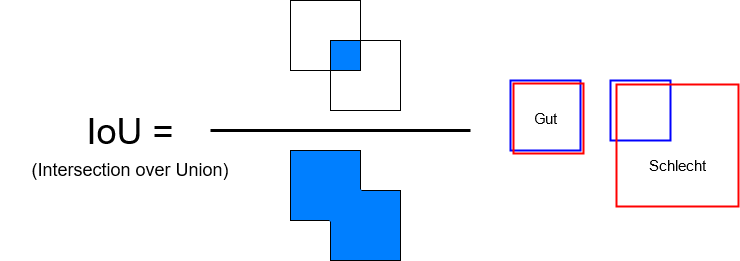
\includegraphics[width=8cm]{Media/Iou.png}
			\caption{Intersection-Over-Union}
			\label{IoU}
		\end{center}
	\end{figure}\\
	In Abbildung \ref{IoU} ist die Berechnung der Intersection-Over-Union dargestellt. Sie beschreibt das Verhältnis der Schnittfläche einer Bounding Box mit der Grundwahrheit bezüglich der Gesamtfläche von Bounding Box und Grundwahrheit. Je genauer die beiden Flächen übereinander liegen desto höher der Wert, desto besser ist die Vorhersage der Bounding Box. ++QUELLE++\\
	\\
	In der zweiten Version von Yolo wurde an mehreren Stellen etwas verbessert. So wurde zum Beispiel Batch-Normalization in Convolutioonal-Layers eingefügt.\\
	Die Inputgröße des Netzes wurde von $224*224$ auf $448*448$ erhöht.\\
	Eine weitere wichtige Änderung sind Ankerboxen. Da Objekte meist immer ähnliche Formen haben kann man eine gewisse Menge an sogenannten Ankerboxen definieren welche als Basis Boundingboxen fingieren. So wird anstatt die absolute Größen von Boxen in Bezug auf das gesamte Bild vorherzusagen, eine Ankerbox ausgewählt die am besten zu dem gewünschten Objekten passende verwendet. Die Abbildung \ref{Anker} zeigt dieses Konzept.
	\begin{figure}[!h]
		\begin{center}
			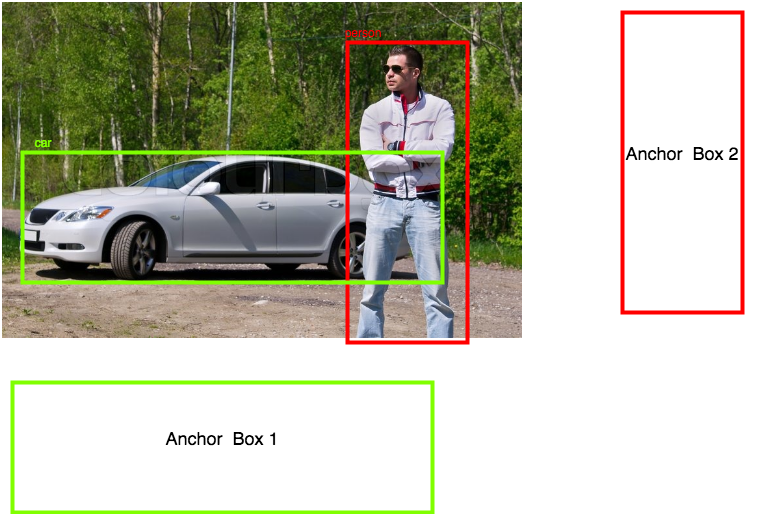
\includegraphics[width=6cm]{Media/Ankerboxen.png}
			\caption{Passende Ankerboxen werden ausgewählt\cite{b0}}
			\label{Anker}
		\end{center}
	\end{figure}
	Diese Ankerboxen kann man mittels Clusteralgorithmen wie K-Means und den Boundingboxen aus dem Datensatz berechnen. Dies hat vor allem den Vorteil das die Boundingboxen besser zu den Objekten des jeweiligen Datensatzes besser passen.\\
	Jede Vorhersagen für eine Boundingbox enthält die 4 Koordinaten: $t_x, t_y, t_w, t_h$. $t_x$ und $ t_y$ sind die x an y Koordinaten, relative Zellen Mittelpunkt. $t_w$ und $ t_h$ sind die Skalierungsfaktoren relativ zu Ankerboxdimensionen. $p_w$ und $p_h$ sind die Breite und Höhe der Ankerbox. Dabei gibt es noch einen Gitterzellenoffset $c_x$ und $c_y$.
	\begin{figure}[!h]
		\begin{center}
			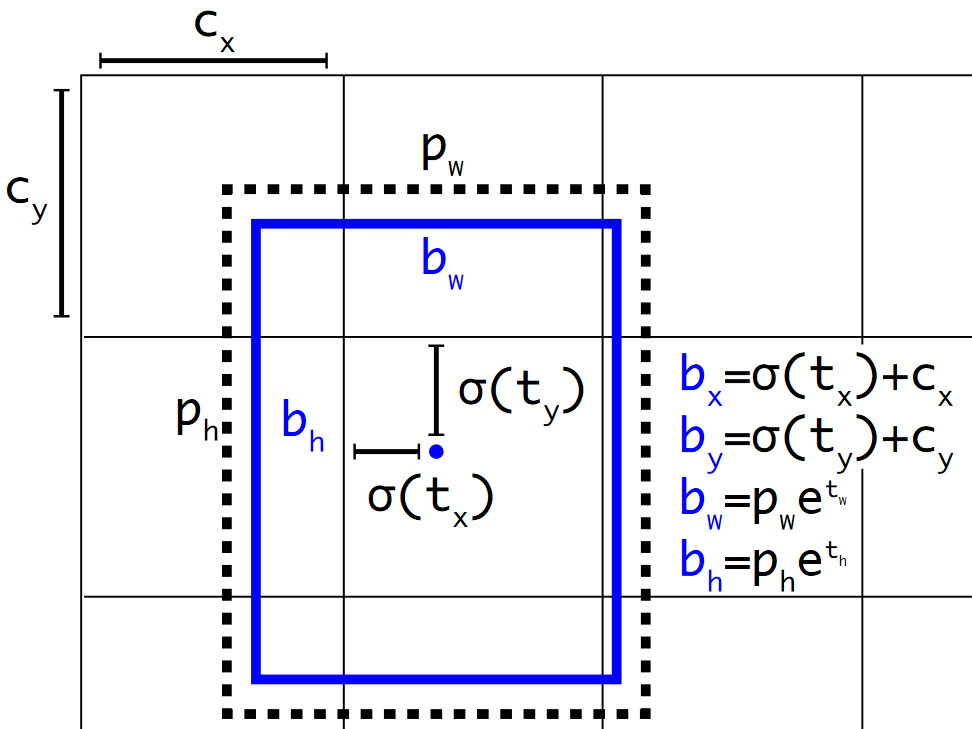
\includegraphics[width=6cm]{Media/YoloV3PredictionBox.png}
			\caption{Zusammensetzung einer Boundingbox\cite{b3}}
			\label{PredictionBox}
		\end{center}
	\end{figure}\\
	Außerdem wir der \textit{objectness score} $t_o$ vorhergesagt.
	\[ P_r(Object)*IoU_{b}^{object} = \sigma(t_o) \]
	$\sigma(t_o)$ entspricht dem Box Konfidenz Score.
	Der Output des Modells enthält für jede Gitterzelle n Boxen, wobei n der Anzahl der Ankerboxen entspricht. Jede Box ist ein Vektor aus 4 Koordinaten objectness score und der Klassen C. Der Vektor enthält: $[b_x,b_y,b_w,b_h, b_o, C]$\cite{b3}.
	\[ C = [c_1, c_2,..., c_{80}]^T\]
	\[ P = [P_r * c_1, P_r * c_2, ..., P_r * c_{80}] \]
	\[ class = argmax_i(C)\]
	\[ score = max(P)\]\\
	In der dritten Version wurde vor allem die Genauigkeit weiter verbessert. So wurden Restblöcke, Skip-Verbindungen und Upsampling Techinken hinzugefügt. Das Netzwerk wuchs damit drastisch auf insgesamt 106 Convolutional-Layer.
	Der Featureextraktor Darknet19 aus YoloV2 wurde durch Darknet-53 ersetzt. Darknet-53 besitzt 53 Convolutional-Layer und beinhaltet zusätzlich vereinzelte Abkürzungen im Netz.\\
	Eine weitere Änderung betrifft den Softmax layer für die Bestimmung der Zielklasse. Früher wurde immer nur die Klasse ausgewählt die den höchsten Score erzielte. Dies hat sich geändert. Dadurch das die Klassenvorhersage mit Hilfe einer Logistische Regession stattfindet kann ein Objekt mehre Label gleichzeitig haben wie zum Beispiel Person und Frau. Diese Multilabelklassifikation wird für unser Projekt aber nicht benötigt.\\
	Ein weitere Neuerung ist das Vorhersagen über drei verschiedene Skalierungen. Das System extrahiert Merkmale mit einem ähnlichen Konzept wie bei Merkmalspyramidennetzen (FPN). Diese Technik verbessert die Genauigkeit vor allem bei kleineren Objekten. So werden Feature-Map aus einer früheren Schicht aus dem Netzwerk extrahiert und mit höher gesampelten Features durch Verkettung zusammen gefügt. Mit weiteren Faltungsschichten werden diese kombinierte Feature-Map verarbeitet. So profitiert man man von Vorhersagen für alle der drei Sklarierungen und damit von allen vorherigen Berechnungen sowie von den feinkörnigen Merkmalen aus der frühen Phase des Netzwerks. Die Abbildung \ref{FPN} zeigt das Konzept eines Merkmalspyramidennetzwerks.
	\begin{figure}[!h]
		\begin{center}
			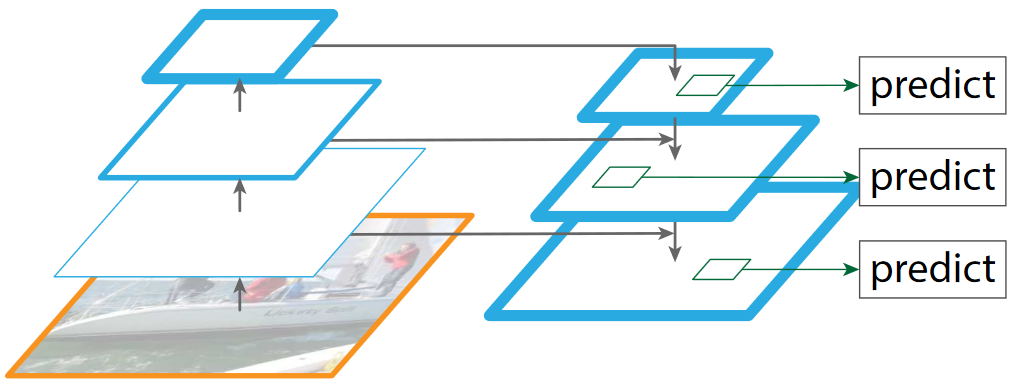
\includegraphics[width=6cm]{Media/FPN.png}
			\caption{Darstellung eines Merkmalspyramidennetzwerks \cite{b6}}
			\label{FPN}
		\end{center}
	\end{figure}\\
	Die letzte dieser Schichten der jeweiligen Skalierungen sagt einen 3-D-Tensor voraus, der Bounding Box, Objekthaftigkeit und Klassenvorhersagen enthält. Es werden aber für jede der drei Skalierung drei Boxen vorausgesagt. Der Tensor entspreche dann für 4 Bounding-Box-Offsets, 1 Objektvorhersage und 80 Klassenvorhersagen $N*N*[3*(4 + 1 + 80)]$.\cite{b4}\\
	\\
	YoloV4 hat die Geschwindigkeit und Genauigkeit verbessert. So nennt das Paper \cite{b2} zum Beispiel \textit{Bag of Freebies}. Damit sind Verbesserungen gemeint die die Genauigkeit des Modells zur Trainingszeit verbessern aber die Inferenzzeit nicht beeinflussen. So wurde stark das Training optimiert. Bei dem Training werden Bilder zusätzlich aus dem Datensatz generiert. Existierende Bilder werden dupliziert und dann rotiert, zugeschnitten, verzerrt, verdunkelt, etc. und dann auch durch das Netz geschickt. 
	Auch Techninken wie \textit{Cut Mix} und \textit{Mosaic Dataaugmentation} werden angewendet. Bei älteren Verfahren werden Bildteile gelöscht. Bei den beiden verwendeten Verfahren werden stattdessen Bildteile aus den Trainingsdaten ausgeschnitten und kombiniert, wobei die Ground-Truth-Labels ebenfalls angespasst werden müssen. Diese Data Augmentation sorgt für eine verbesserte Generalisierungfähigkeit des Modells.\\
	Regularisierungmethoden wie \textit{DropOut}, \textit{DropConnect} und \textit{DropBlock} wurden gegen Overfitting eingesetzt.\\
	Auch wird die Lossfunktion angepasst. Bei den bisherigen Versionen wurde die Mittlere quadratische Abweichung (MSE) für das Regressionsproblem verwendet. Diese Regression wird dann unabhängig für alle Vorhersagen von $t_x, t_y, t_w, t_h$ verwendet. Sinnvoller ist es die Koordinaten zusammen als die IoU der Boundingboxen in Betracht zu ziehen. Deshalb verwendet YoloV4 \textit{CIoU} als Lossfunktion um die Integrität der Objekte mit einzubeziehen.
	Weitere Verbesserungen die auf Kosten der Laufzeit gehen werden \textit{Bag of Specials} genannt. Dazu gehören zum Beispiel \textit{Squeeze-and-Excitation}, \textit{Spatial Attention Module}, Vergrößerung des Rezeptionsfeldes des Modells und Stärkung der Fähigkeit zur Merkmalsintegration.\\
	Im Backbone wird eine \textit{MISH}-Aktivierungsfunktion verwendet. Diese ist eine glatte und nicht-monotone neuronale Aktivierungsfunktion, die wie folgt definiert werden kann:
	\[ f(x) = x* \tanh (\ln (1+e^x)) \]
	Sie arbeitet besser als zum Beispiel \textit{ReLU} oder Swish \cite{b7}.\\
	Die Komponenten in der Architektur wurde auch ersetzt. Im \textit{Backbone} läuft nun \textit{CSPDarknet53}. Dies basiert auf dem Darknet53 aus YoloV3 und wird mit Cross-Stage-Partial-Networks erweitert. Im Hals des Netzes wird \textit{Spatial pyramid pooling} (SPP), \textit{Path Aggregation Network} (PANet) und \textit{Spatial Attention Module} (SAM) statt den Merkmalspyramidennetzen (FPN) aus YoloV3 verwendet.\\
	SPP wendet verschiedene Strategien bei unterschiedlichen Skalierungen an. Sie ersetzt den letzte Pooling-Layer durch einen räumlichen Pyramiden-Pooling-Layer. Die Feature-Maps werden räumlich in $m$ × $m$ Bins unterteilt. In Yolo wird eine modifiziert Version von SPP verwendet die die räumliche Dimension der Ausgabe beibehalten.
	In FPN werden die Objekte separat und unabhängig voneinander auf verschiedenen Skalenebenen erkannt. Dies kann zu doppelten Vorhersagen führen. PAN kombiniert deshalb die Informationen aus allen Ebenen.\\
	SAM verbessert die räumliche Aufmerksamkeit.\\
	Am \textit{Head} der für Prädiktion verantworlich ist wurde nichts geändert und  ist damit identisch zu YoloV3 \cite{b2}\cite{b8}. Diese Architektur mit der viel zahl an Komponenten wird in er Abbildung \ref{V4Arch} dargestellt.
	\begin{figure}[!h]
		\begin{center}
			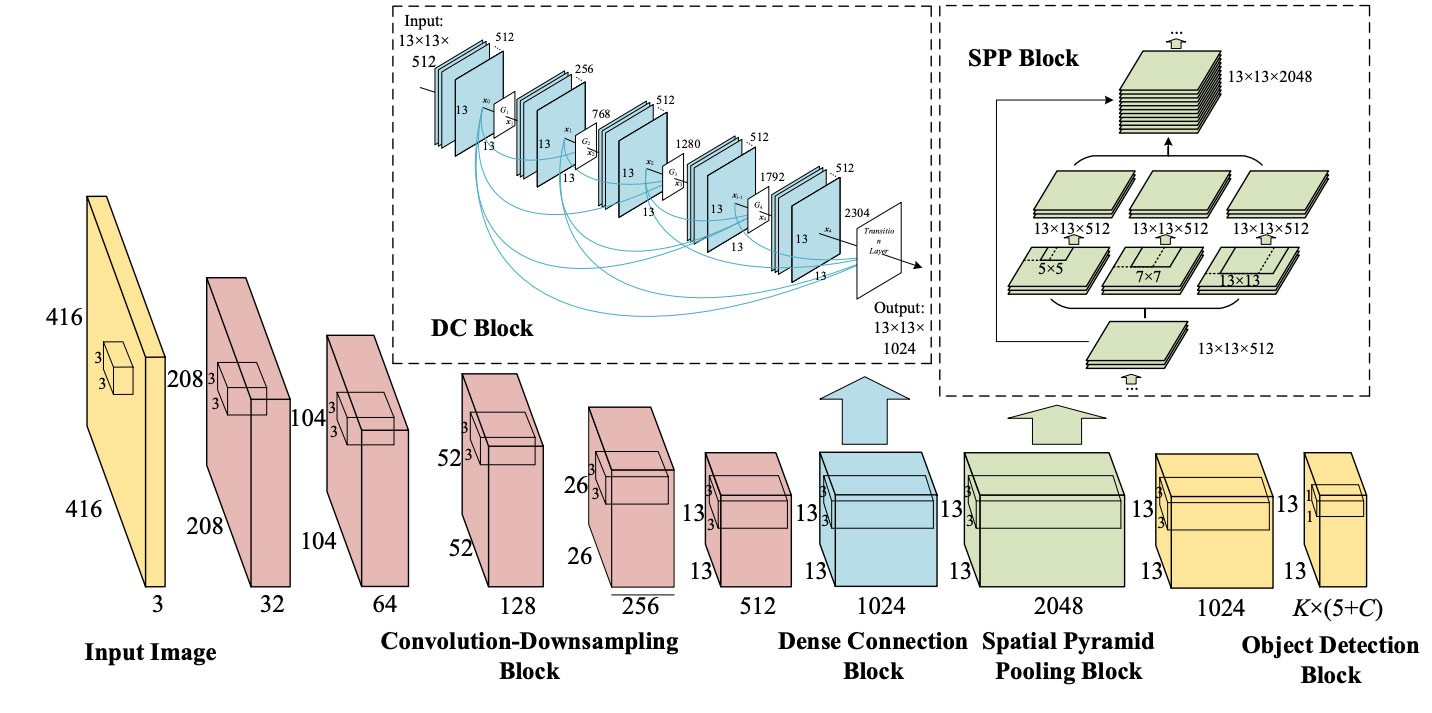
\includegraphics[width=9cm]{Media/YoloV4Arch.jpeg}
			\caption{Das Konzept von YoloV4 \cite{b8}}
			\label{V4Arch}
		\end{center}
	\end{figure}\\
	Wir mussten unser Modell nicht mehr trainieren da es bereits mit dem Microsoft COCO Datensatz trainiert wurde. Es sind 80 verschiedene Klassen erkennbar. Wir interessieren uns aber nur für einen kleineren Teil wie:
	\begin{enumerate}
		\item Personen
		\item Pkw
		\item Lkw
		\item Busse
		\item Fahrräder
		\item Züge
	\end{enumerate}
	Das Modell könnte noch besser arbeiten wenn es nur auf die Klassen trainiert würde die für unser Projekt relevant sind. Dies hätte aber den Rahmen des Projektes gesprengt. Das Modell ist mit ein paar Ausnahmen für das Projekt ausreichend gut genug.\\
	Dennoch kann man je nach Szenario per Parameter die relevanten Klassen auswählen. Das Modell prädiktiert trotzdem noch alle Klassen. Die nicht relevanten werden einfach nur im Postprocessing herausgefiltert.\\
	Ein weitere Postprocesingschritt ist es die Detektion die eine zu geringe Sicherheit besitzen zu entfernen.\\
	Die übrigen Boxen durchlaufen eine Non-Maxima-Suppression.
	Der Output kann überschneidende Boundingboxen besitzen die eigentlich zur selben Klasse gehören. Diese Duplikate können mittels der Non-Maxima-Suppression entfernt werden. Hierfür wird die IOU der Boxen berechnet. Sollte die IOU einen Threshold überschreiten dann wird das Duplikat entfernt. Die Grafik \ref{NMS} zeigt wie zu viele überlappende Boxen mit einer NMS mit einer ersetzt werden kann.\\
	\begin{figure}[!h]
		\begin{center}
			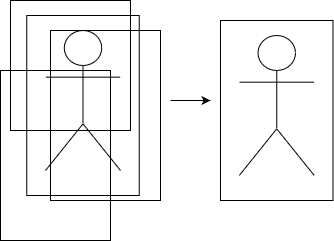
\includegraphics[width=6cm]{Media/NMS.png}
			\caption{Non-Maxima-Suppression}
			\label{NMS}
		\end{center}
	\end{figure}\\
	Das Ergebnis einer Prädiktion ist eine Liste von Objekten welches aus den x,y Koordinate des Mittelpunktes der Boundingbox, der Breite w, der Höhe h, der Klasse und des Konfidenzwerts besteht.
	
	\subsection{Fehler in der Erkennung}
	ZUG FEHLT+++++++++++\\
	YoloV4 ist nicht perfekt. So gibt es gelegentlich Fehler:
	\textbf{Falschklassifizierung:}\\
	Selten Klassifiziert das Netz falsch. So wie in der Abbildung \ref{FaK} zu sehen ist wurde ein Bus als Pkw klassifiziert. Das Modell ist sich in diesem Beispiel auch nur unsicher mit $31\%$. Der Fehler lässt sich vermutlich erklären da die Frontpartie des Bus einem Pkw sehr ähnelt und der Rest des Fahrzeuges wegen einem Baum und einer Laterne verdeckt wird. Auch ist zu vermuten, dass das Netz falsche Merkmale gelernt hat. Dies könnte mit Sicherheit verbessert werden wenn das Modell nur auf die für uns relevanten Klassen trainiert worden wäre. Die folgenden Abbildungen \ref{FaK}, \ref{FaK2}, \ref{FaK3} und \ref{FaK4} sind Beispiele für falsche Klassifikationen. Speziell ist vorallem der Fehler in Bild \ref{FaK4}. Hier wurde ein Anhänger als Fahrzeug klassifiziert. Der Ursprung dieses Fehlers kann unterschiedliche Gründe haben. Dies liegt wahrscheinlich auch am Datensatz selbst.
	\begin{figure}[!h]
		\begin{center}
			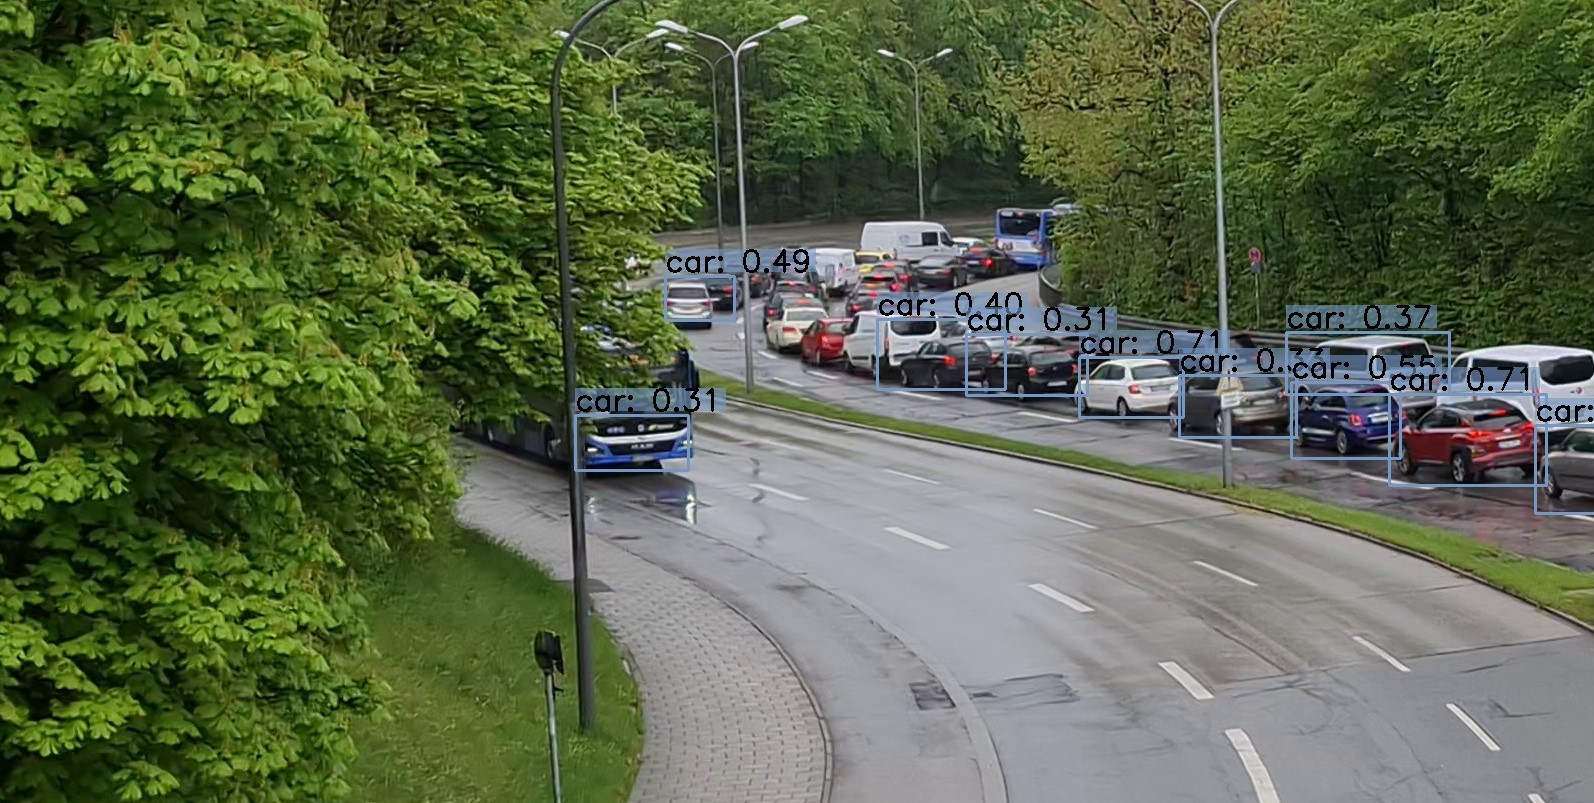
\includegraphics[width=7cm]{Media/Output_480 - Kopie.jpg}
			\caption{Falschklassifizierung eines Bus wegen Verdeckung}
			\label{FaK}
		\end{center}
	\end{figure}\\
	\begin{figure}[!h]
		\begin{center}
			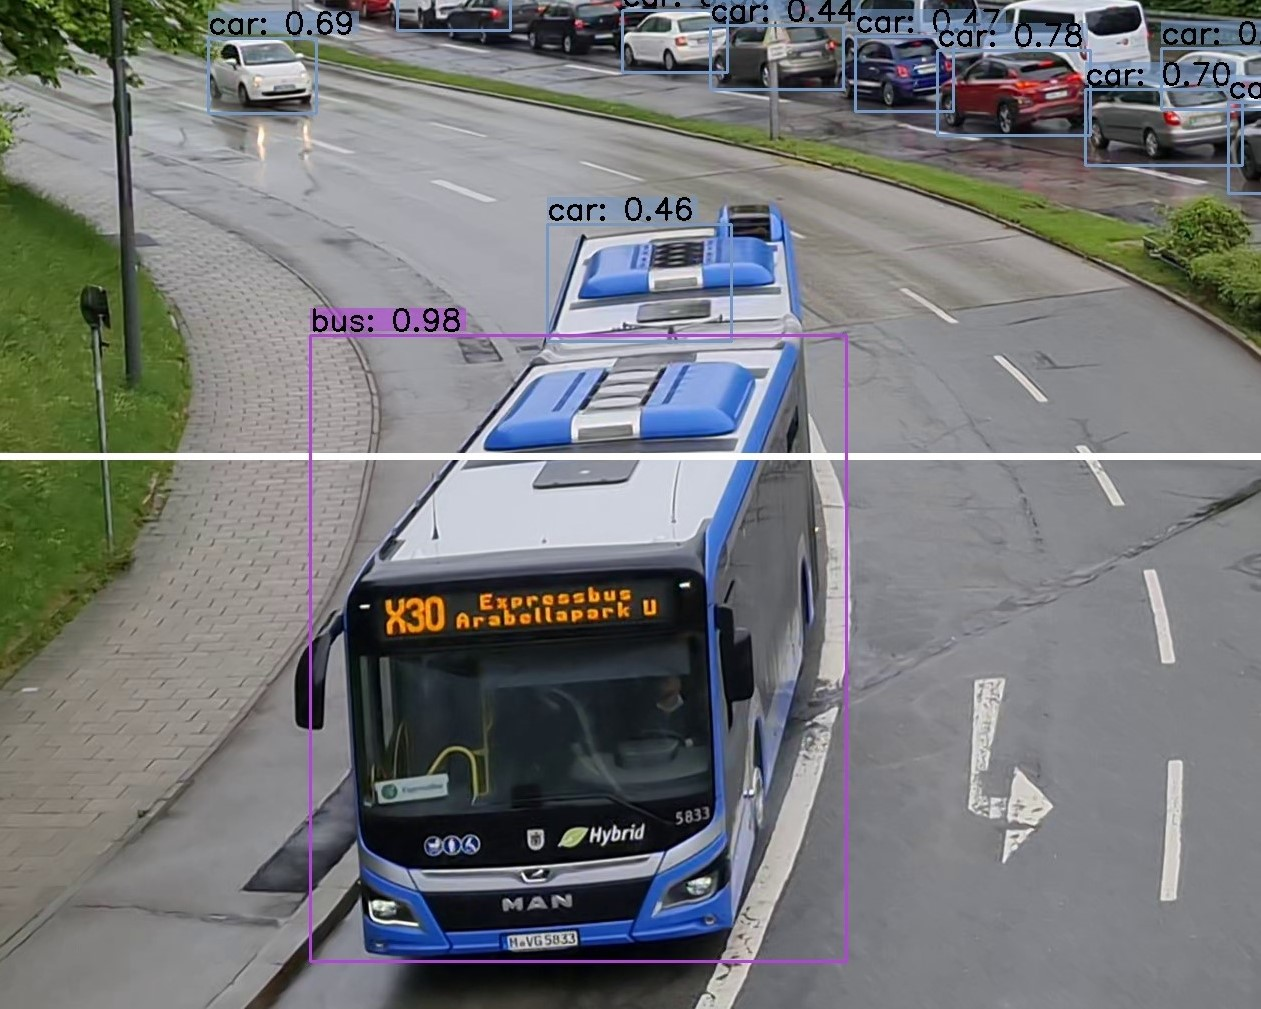
\includegraphics[width=7cm]{Media/Output_847 - Kopie.jpg}
			\caption{Falschklassifizierung des Dachs als Pkw}
			\label{FaK2}
		\end{center}
	\end{figure}\\
	\begin{figure}[!h]
		\begin{center}
			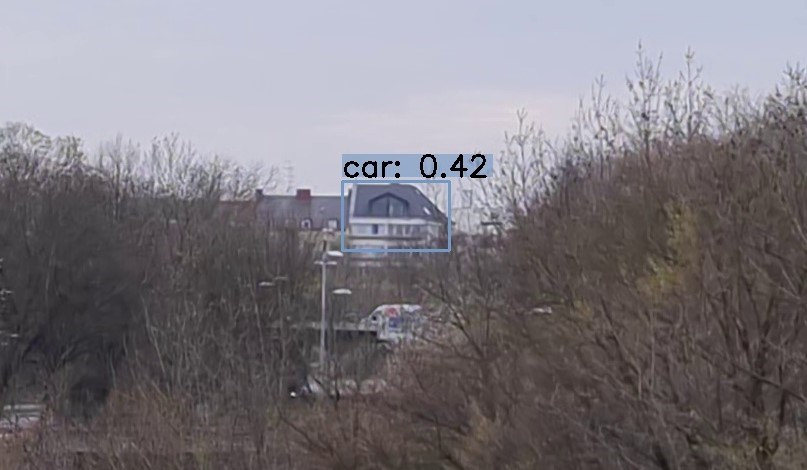
\includegraphics[width=7cm]{Media/Output_108 - Kopie (2).jpg}
			\caption{Falschklassifizierung eines Hausdachs}
			\label{FaK3}
		\end{center}
	\end{figure}\\
	\begin{figure}[!h]
		\begin{center}
			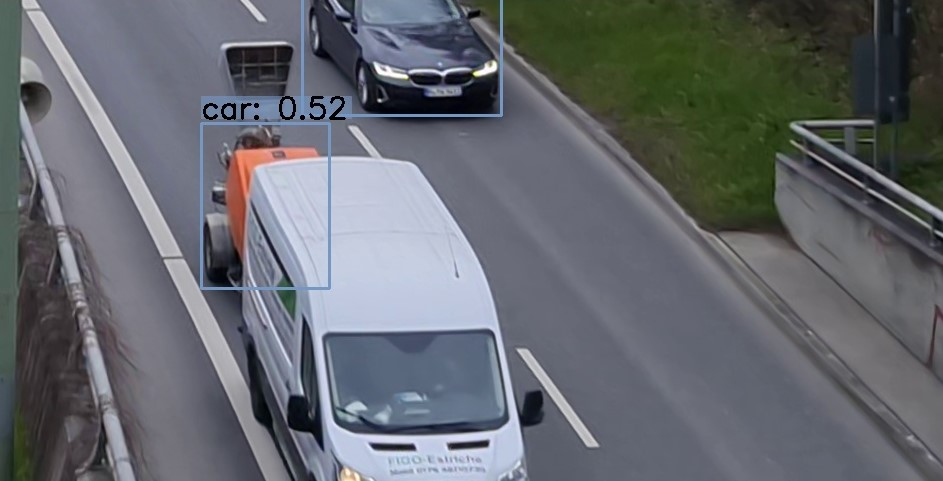
\includegraphics[width=7cm]{Media/Output_829 - Kopie.jpg}
			\caption{Falschklassifizierung eines Anhängers}
			\label{FaK4}
		\end{center}
	\end{figure}\\
	
	\textbf{Fehlende Detektion:}\\
	Ein etwas häufigerer Fehler ist das Detektionen komplett fehlen. Dies kann mehrere Gründe haben. So zeigt die Abbildung \ref{FeK} zwei Typische Gründe. Hauptgrund ist es das Objekte teilweise verdeckt sind. In Kombination wenn Objekte sehr klein sind ist es nahezu nicht mehr möglich zuverlässig Detektion zu bekommen. Auch wenn Objekte das Bild verlassen oder gerade betreten kann es noch kurz zu fehlenden Detektionen führen.
	\begin{figure}[!h]
		\begin{center}
			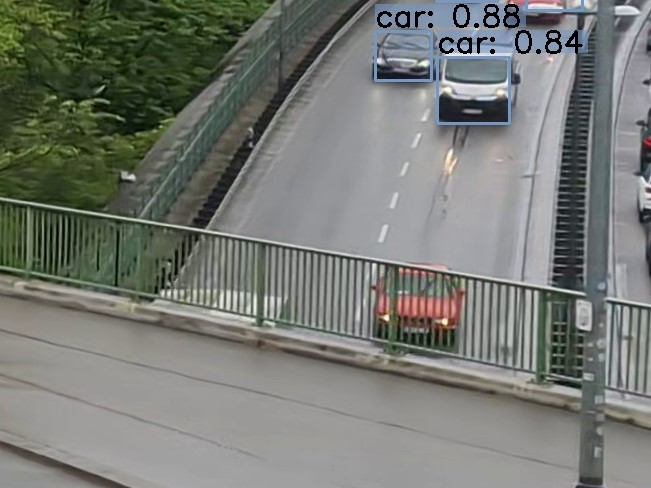
\includegraphics[width=7cm]{Media/Output_680 - Kopie.jpg}
			\caption{Fehlende Klassifikationen}
			\label{FeK}
		\end{center}
	\end{figure}\\
	\begin{figure}[!h]
		\begin{center}
			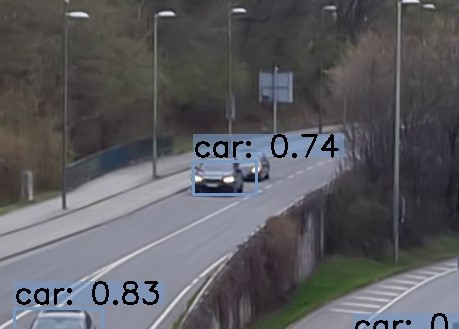
\includegraphics[width=7cm]{Media/Output_108 - Kopie.jpg}
			\caption{Fehlende Klassifikationen}
			\label{FeK2}
		\end{center}
	\end{figure}\\
	\textbf{Unpassende Boundingboxen:}\\
	Yolo hat durch seine Eigenschaf nur rechteckige Boundingboxen vorhersagen zu können eine große Schwäche. Das resultiert in manchen Szenarien zu sehr unpassenden Boundingboxen. Beispielsweise kann man in der Abbildung \ref{UB} gut erkennen das wegen dem Busses welcher Diagonal steht die Boxen zu groß werden. Der Effekt tritt noch verstärkter auf bei  noch längere Objekte wie die Zügen.++++++++ZUG BILD++. Auch kann die Box für das Objekt etwas falsch anliegen wenn Bäume oder Laternen ein Teil verdecken wie in Abbildung \ref{UB2} zu sehen ist. Diese unpassenden Boxen erschweren das Tracking ungemein. Dazu später aber noch mehr.
	\begin{figure}[!h]
		\begin{center}
			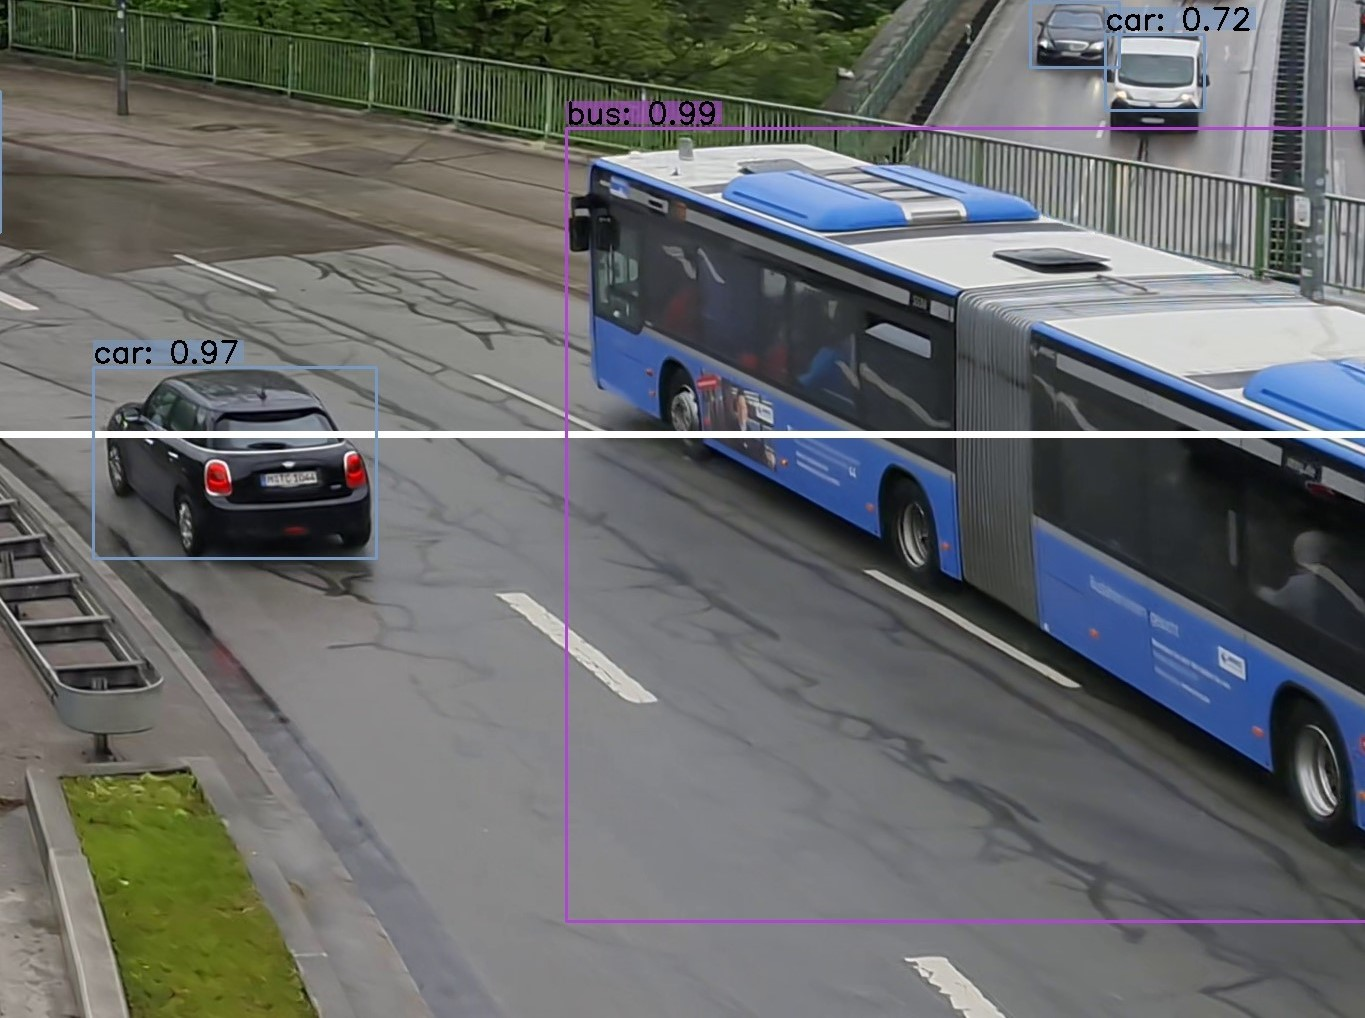
\includegraphics[width=7cm]{Media/Output_777 - Kopie.jpg}
			\caption{Unpassende Boundingboxen}
			\label{UB}
		\end{center}
	\end{figure}\\
	\begin{figure}[!h]
		\begin{center}
			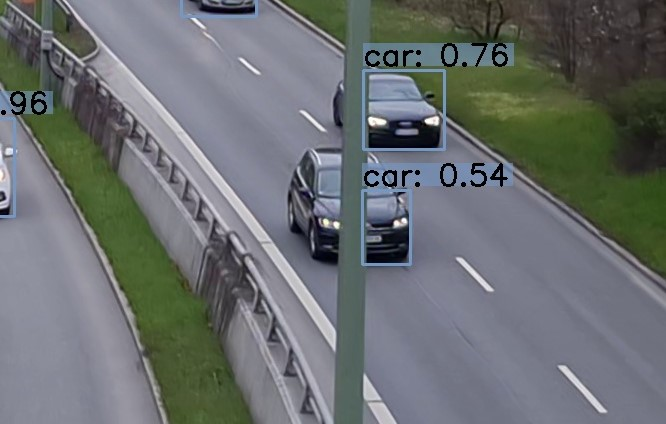
\includegraphics[width=7cm]{Media/Output_276 - Kopie.jpg}
			\caption{Unpassende Boundingboxen}
			\label{UB2}
		\end{center}
	\end{figure}\\
	
	\section{Tracking: Sort}
	SORT berechnet auf Basis des Kalman Filters und der Hungarian Methode die Bewegung des Objekts und weist je nach Status eine eindeutige Identifikationsnummer zu. Die Hungarian Methode, auch Kuhn-Munkres-Algorithmus genannt, wird für das Lösen von Zuordnungsproblemen in einem gewichteten kompletten bipartiten Graph genutzt. Hierbei wird die Zuordnung anhand der minimalen Gewichtung, zwischen den Elementen gelöst. Gegeben ist ein Graph $G = (A \cup B, E) $. Zwischen $A$ und $B$ wird nun die Verbindung mit der kleinsten Gewichtung gesucht. Hierfür wird eine Kostenmatrix $C$ erstellt mit $c_{ij}$ als Kosten um $a_i \in A$, $b_j \in B$ zuzuordnen. 
	
	Der Kalman-Filter funktioniert für die Problemstellung sehr gut, da dieser ein lineares System mit gaußisches Rauschen voraussetzt. Dies ist gegeben durch die gleichmäßige Bewegung der Züge/ Autos in eine Richtung.
	Der Kalmanfilter kann aus verrauschten, teils redundanten Messungen die Zustände und Parameter des aktuellen Systems schätzen. 
	Die Zustände des aktuellen Systems sind die Positionen der Objekte angegeben in Bounding Boxen. Durch Berücksichtigung des letzten Zustand des Systems, (die letzte Position), der Schätzung der nächsten Position und Abgleich mit der aktuellen Messung (die aktuelle Detektion) und anschließender Aktualisierung des Systems, kann eine zuverlässige Verfolgung des Objekts berechnet werden. Probleme die den Kalmanfilter stören sind zum Beispiel ungleichmäßige Bewegungen von Fahrzeugen, dies wird „Process Noise“ genannt, sowie Ungenauigkeiten in Messungen, diese werden als „Measurement Noise“ bezeichnet.
	Kann zu dem aktuell getrackten Objekt in dem Frame keine Bounding Box zugeordnet werden, wird der Zustand des Systems auch ohne die Korrektur durch die Messung berechnet. Kann in einem späteren Frame wieder eine Bounding Box zugeordnet werden, wird der Zustand durch diese Detektion erneut aktualisiert. 
	Die Hungarian Methode wird verwendet, um die Detektion einem existierenden getrackten Objekt zuzuordnen. Hierfür wird die Intersection-over-Union Distance zwischen jeder Detektion und allen bereits erkannten Objekten verglichen und als Gewichtung verwendet.
	
	
	
	Die Zuweisung der ID erfolgt anschließend über die optimale Lösung der Hungarian Methode.
	
	\section{Tracking: DeepSort}
	
	SORT an sich ist bereits ein Tracker, das Problem ist jedoch, dass die ID-Änderungen zu oft auftreten. Das heißt die Objekt-ID wechselt während der Verfolgung. Ausgelöst wird dies zum Beispiel durch die teilweise Verdeckung des Objekts. Deshalb wurde SORT um ein CNN erweitert, welches sowohl einerseits die Mahalanobis-Distanzmetrik für die Assoziation nutzt, als auch die Form des Objekts in Form eines durch das hinzugefügte CNN berechneten Feature-Vektor verfolgt. Durch Verwendung einer geeigneteren Distanzmetrik und Beschreibung des Objekts kann dieses nun besser verfolgt werden.
	Das CNN erstellt einen Vektor, der enthält alle Features eines gegebenen Bilds. Ursprünglich wird das Neuronale Netz als Klassifikator trainiert. Indem die Klassifikations Layer weggelassen werden, können die resultierenden Feature-Vektoren als Wiedererkennungsform verwendet werden.
	
	Anstatt bei der Ungarischen Methode wie bei SORT die IoU-Distanz zu verwenden, wird nun die (quadrierte) Mahalanobis Distanz verwendet, welche die Distanz zwischen der detektierten Bounding Box und der gaußverteilten Vorsage des Zustands des Kalman-Filters berechnet:
	\begin{align}
		d^{(1)}(i,j)= (d_j - y_i)^TS^{-1}_i(d_j - y_i)
	\end{align}
	Hierbei wird die Verteilung, zuvor acht-dimensional des i-ten verfolgen Objekts in den vier-dimensionalen Raum der Messungen projiziert $(y_i, S_i)$. Diese Bounding Box der Detektion wird mit $d_j$ bezeichnet. \\
	
	
	\begin{tabular}{r l}
		Kalman-Filter Zustand: & $(u,v,\gamma,h,\dot{x},\dot{y},\dot{\gamma},\dot{h})$ \\
		Detektion: & $(u,v,\gamma,h)$ \\
		$u,v$ :& Mittelpunkt der Bounding Box \\
		$h$ :& Skalierungsfaktor \\
		$\dot{x},\dot{y},\dot{\gamma},\dot{h}$: & Geschwindigkeiten in Bild- \\	
		& koordinaten \\
	\end{tabular} \\
	
	Die Mahalanobis Distanz berechnet den Abstand von einem Punkt zu einer Verteilung. Der Abstand ist dabei wie viele Standardabweichungen der Verteilung dieser Punkt vom Mittelwert der Verteilung entfernt ist. Er wird somit durch die Standardabweichung der Verteilung normiert. Die Detektion stellt hierbei den Punkt da und die Unsicherheit der Zustandsvorhersage, beziehungsweise die Unsicherheit der Position des getrackten Objekts, die Verteilung. Dadurch wird bei der Berechnung der Distanz die Unsicherheit der Position miteinbezogen.
	
	Für die Distanzmetrik ergibt sich dann folgende Gleichung
	$D = \lambda * D_k + (1-\lambda) * D_a$. Hierbei ist $D_k$ die Mahalanobis Distanz und $D_a$ die kleinste Kosinus-Distanz zwischen den Feature-Vektoren. $\lambda$ dient als ein Gewichtungsfaktor.
	
	Kann DeepSORT erfolgreich ein bereits verfolgtes Objekt zu einer Detektion assoziieren, wird anschließend eine TrackingID erstellt. Hierbei muss beachtet werden, dass im Zuge der Verbesserung von SORT weitere Sicherheiten eingebaut wurden. Ein neu getracktes Objekt erhält nicht sofort eine endgültige Identifikationsnummer. Erst nachdem das Objekt in drei hintereinander liegenden Frames erfolgreich getrackt werden konnte erhält es eine Nummer. Das Objekt erhält des weiteren einen Zähler $a$, der die Anzahl an Frames zählt, seitdem das Objekt nicht mehr erfolgreich assoziiert werden konnte. Ist eine maximale Anzahl $Age_{max}$ erreicht gilt das Objekt als verloren oder außer Reichweite der Kamera und wird aus der Objektliste entfernt. Dieser Zähler wird jedoch zurückgesetzt, sollte zuvor das Objekt erneut erfolgreich assoziiert werden.
	
	\section{Zählen von Objekten}
	Wir testeten verschiedene Verfahren zu Zählen der gefundenen Objekte die das Video passieren.\\
	\textbf{Zählen der vergebenen TrackingID's.} Unser erster Plan war das Zählen aller vergebenen Tracking ID's. Dies hätte den Vorteil das sobald ein Objekt gefunden wird auch gezählt wird. Wir stellten aber schnell fest das Aufgrund von Fehlern in der Pipeline Objekten mehrfach neue IDs zugewiesen wurde. Diese Probleme entstehen in Kombination aus Fehlern in der Objekterkennung und dem Tracker. Je zuverlässiger das Tracking funktioniert desto geringer ist der Fehler im Zählen. Da aber ein perfekter Tracker nicht immer realistisch ist müssen bessere Lösungen gefunden werden.\\
	\textbf{Zähllinie.} Um Trackingfehler zu umgehen bauten wir eine Zähllinie ein die sobald der Mittelpunkt der Boundingbox diese schneidet einmal hochzählt. Dies hatte noch immer Probleme wie zum Beispiel das manche Boxen doppelt gezählt wurden ohne manche die Linie direkt übersprungen haben. WAS WAR DA NOCHMAL FALSCH Thomas?\\
	\textbf{Zählung der Tracking IDs in einer Zählbox.} Um die beiden Techniken zu vereinen wurde eine Zählbox entwickelt. So kann für jedes Szenario per Parameter die Position und Größe der Zählbox definiert werden. Sobald der Mittelpunkt einer Boundingbox in den die Zählbereich eindringt wird überprüft ob diese Tracking ID schon in einem Set enthalten ist. Ist sie es noch nicht wird hochgezählt. Es ist sinnvoll die Zählbox in Bereiche zu setzten in denen das Tracking zuverlässig funktioniert. 
	\begin{figure}[!h]
		\begin{center}
			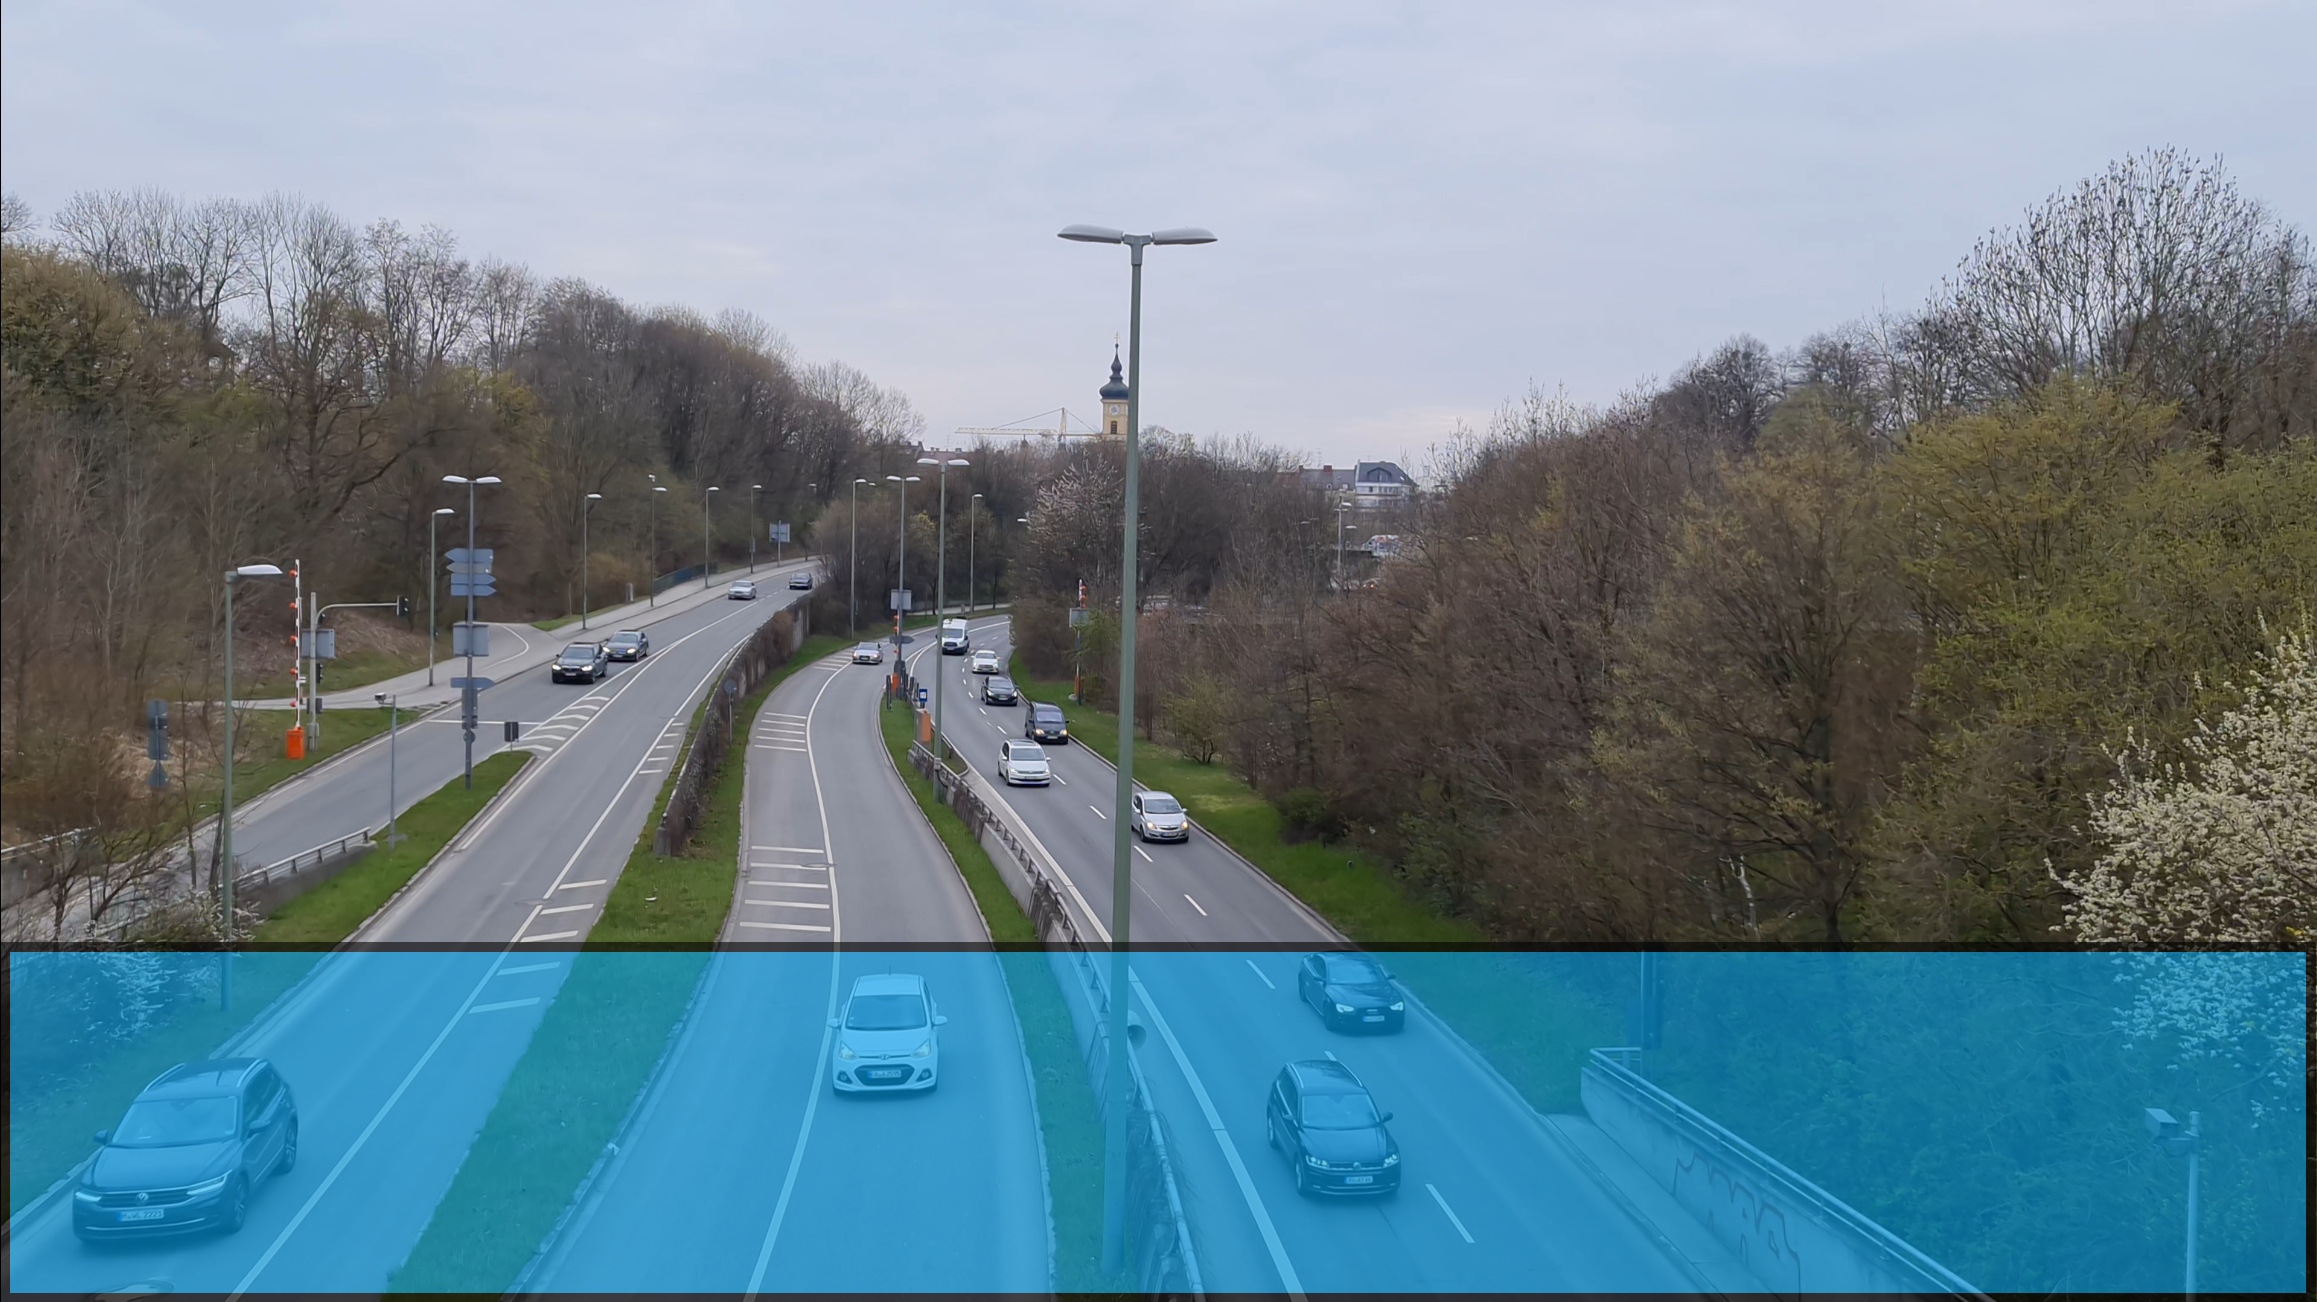
\includegraphics[width=7cm]{Media/BrudermuhlCounter.png}
			\caption{Darstellung einer Zählbox}
			\label{Counter}
		\end{center}
	\end{figure}
	
	\section{Zustandserkennung Züge}
	Da nun ein Objekt erfolgreich erkannt, verfolgt und seine Bewegungsrichtung erkannt werden kann, wird nun für Objekte die der Klasse Zug zugeordnet sind, die aktuelle Zugphase bestimmt.  
	Durch YOLO werden die Bounding Boxen pro Frame bestimmt. Durch Abgleich der TrackingID kann festgestellt werden, ob es sich immer um den selben Zug handelt. Für jede der Detektionen des ausgewählten Zugs wird durch Optical Flow die Magnitude und die Richtungswinkel bestimmt. Dabei wurde die durchschnittliche Richtung über die gesamten Richtungsvektoren der Bounding Box des Zuges bestimmt. Dies wurde im Verlauf des Projekt durch die Richtungsbestimmung des Kalmanfilters ersetzt. Dieser berechnet zusammen mit dem nächsten Zustand auch die den Richtungsvektor. Fährt der Zug ein, hat dieses Objekt durch die Bewegung eine Magnitude größer 1. Der Richtungsvektor wird zur Visualisierung in das Bild als Pfeil eingefügt. Sobald der Zug erkannt wird und eine Richtung bestimmt wird, wechselt dessen Zustand von „Kein Zug“ zu „Einfahrend“. Dabei wird immer für 5 Frames geprüft ob die Richtung gleichbleibend ist. Sollte für eine Länge von 10 Frames die Magnitude unter 0 fallen ändert sich der Zustand des Zuges zu „Haltend“. Beginnt der Zug sich wieder zu bewegen und die Bewegung ist gleichbleibend in eine Richtung wird der Zustand auf „Abfahrend“ gesetzt, bis der Zug außerhalb des Bildes ist und nicht mehr erkannt wird.
	
	
	
	\section{Vergleich klassischen Methoden mit Deep-Learning}
	\textbf{Eigenschaften der klassischen Verfahren:}
	\begin{itemize}
		\item Klassische Verfahren sind deutlich besser nach zu vollziehen. Dies gilt vor allem für Fehler....
		
		\item Klassische Verfahren sind deutlich schneller. Diese Verfahren sind um den Faktor X schneller als DeepLearningverfahren...........
		
		\item Klassische Verfahren können auch gute Leistung erzielen mit genug feinschliff......
	\end{itemize}
	
	\textbf{Eigenschaften der Deep-Learning Verfahren:}
	\begin{itemize}
		\item Deep-Learning Verfahren sind deutlich schlechter nach zu vollziehen. Dies gilt vor allem für Fehler....
		
		\item Klassische Verfahren sind deutlich schneller. Diese Verfahren sind um den Faktor X schneller als DeepLearningverfahren...........
		
		\item Die Deep-Learning Verfahren verzeichnen vorallem gute Out-Of-The-Box Leistung. 
	\end{itemize}
	
	\begin{thebibliography}{00}
		\bibitem{z1}https://www.zeit.de/news/2020-10/18/s-bahn-stammstrecke-in-muenchen-fuer-arbeiten-gesperrt
		\bibitem{b0}https://medium.com/@sarangzambare/object-detection-using-non-max-supression-over-yolov2-382a90212b51
		\bibitem{b1}https://arxiv.org/pdf/1506.02640v5.pdf
		\bibitem{b2}https://arxiv.org/pdf/2004.10934.pdf %V4
		\bibitem{b3}https://arxiv.org/pdf/1612.08242.pdf %V2
		\bibitem{b4}https://pjreddie.com/media/files/papers/YOLOv3.pdf %V3
		\bibitem{b5}https://jonathan-hui.medium.com/real-time-object-detection-with-yolo-yolov2-28b1b93e2088 % V1 Loss
		\bibitem{b6}https://openaccess.thecvf.com/content\_cvpr\_2017/papers/Lin\_Feature\_Pyramid\_Networks\_CVPR\_2017\_paper.pdf % FPN
		\bibitem{b7}https://arxiv.org/vc/arxiv/papers/1908/1908.08681v1.pdf%MISH
		\bibitem{b8}https://jonathan-hui.medium.com/yolov4-c9901eaa8e61 %Yolov4 Hui
	\end{thebibliography}
	
	\section{Anhang}
	
	
\end{document}
